\section{Design and manufacturing of quadrotor} 

The main body of the drone is created as a PCB, in order for the body to host both the structural element and the electrical connections of the drone. Since the project formulation’s main goals dictates the drones size and mechanical properties, the drones size was chosen to be $100 mm^2$, so that the PCB could accommodate all the needed components of the drone. The PCB shape itself was designed in Siemens NX as a simple outline with holes for the motor mounts. This outline was exported in a DXF format into Autodesk Eagle were the actual PCB was designed from the needed electrical circuit. The electrical schematic was created in Eagle’s schematic designer and then automatically converted to a PCB board with the auto-router feature. The trace width of the PCB is specifically chosen to be 30 mills so it can supply the needed 1.72 amps \cite{PCBTracewidth} for the motors at maximum rpm. The microcontroller of the drone is mounted by pin headers, the motors by the motor mounts and the remaining components by soldering onto the top layer. The position of the microcontroller is offset from the center, in order to ensure that the In-built 6-axis IMU is centered to the exact middle of the PCB.

\begin{figure}[H]%
    \centering
    \subfloat[\centering CAD View]{{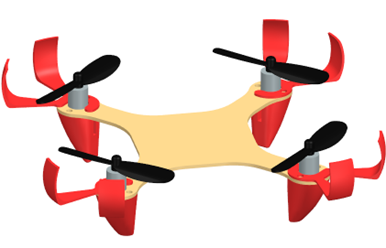
\includegraphics[width=5cm]{design/DroneCAD.png} }}%
    \qquad
    \subfloat[\centering PCB View]{{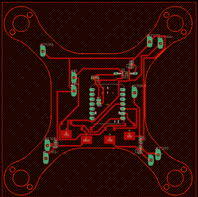
\includegraphics[width=5cm]{design/PCBpicture.png} }}%
    \caption{Drone model}%
    \label{fig:example}%
\end{figure}

In order to control the speed of the motors, one of the potential options would be to use an H-bridge to control
the DC motors. However that would be excessive, as the motors does not need to run in reverse as contain many components
As a less power consuning simple and lighter option, a single N-channel mosfet was used for each motor.

\begin{figure}[H]
    \begin{center}
    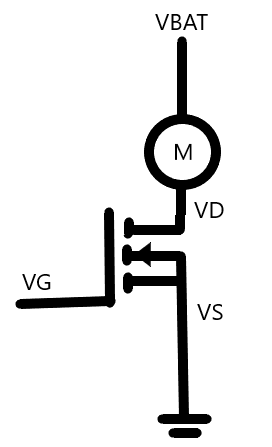
\includegraphics[width=5cm]{design/Mosfet_Control}
    \end{center}
    \caption{Motor control with MOSFET.}
    \label{fig:Mosfet_Control}
\end{figure}

As illustrated in figure \ref{fig:Mosfet_Control}, the drain of the MOSFET is connected to the motor, which is supplied by 
the battery, and the source of the MOSFET is grounded. Meanwhile, the VG pins are connected to one of the PWM pins 
of the nRF52840 MCU, where the opening of the gate is proportional to the PWM. Thus, when VG (simulated by PWM) is 
smaller than the V threshold of the MOSFET, the motors are static, and if VG surpasses V threshold, then the motors 
start spinning with higher RPM as PWM is increased. 
The MOSFETs used for this situation are FDD8896 \cite{FDD8896}, as it has 
a low threshold voltage of 2.5V (MCU pins can supply 
up to 3.3V), and can handle up 94A in continuous drain 
current.

As there is high currents being drawn from the motors, one of the things needed to be configured was protection 
against overcurrent being drawn from the microcontroller. When the motors are switched on or off, 
a surge current arises which can result in additional overcurrent being pulled from the microcontroller if 
the battery is not alone capable of supplying the current. 


\begin{figure}[H]%
    \centering
    \subfloat[\centering Continuous Current]{{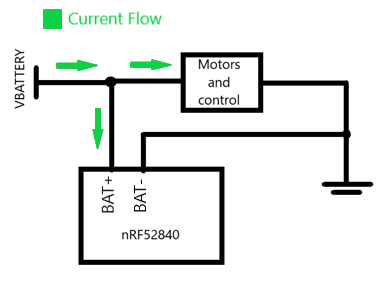
\includegraphics[width=5cm]{design/Continuous_Current} }}%
    \qquad
    \subfloat[\centering Potential Surge current]{{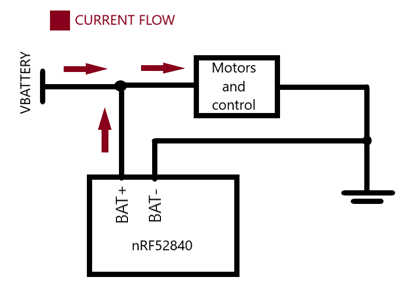
\includegraphics[width=5cm]{design/Surge_Current} }}%
    \caption{Current flows}%
    \label{fig:example}%
\end{figure}


In order to prevent reverse current from the MCU, 
during a surge, one of the potential options to utilise would be a diode placed in the following 
configuration. 

\begin{figure}[H]
    \begin{center}
    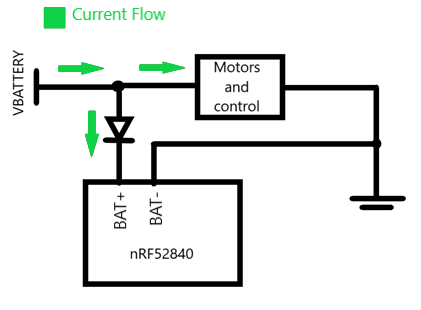
\includegraphics[width=5cm]{design/Diode_Protection}
    \end{center}
    \caption{Diode added to prevent reverse current flow from MCU.}
    \label{fig:Diode_Protection}
\end{figure}

Additionally decoupling capacitors were added in 
parallel to the positive and negative motor pins 
and the MCU BAT+ and BAT- pins.

\begin{figure}[H]
    \begin{center}
    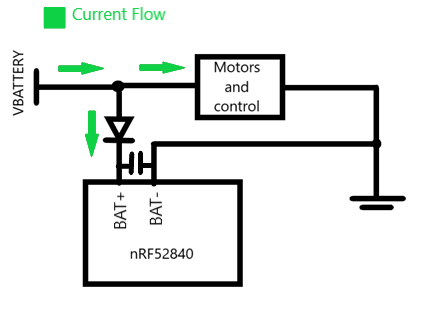
\includegraphics[scale=0.7]{design/Diode_Protection_&_decoupling_capacitors}
    \end{center}
    \caption{Example of decoupling capacitor for stable voltage to MCU.}
    \label{fig:Diode_Protection_&_decoupling_capacitors}
\end{figure}

The diode utilised is 1N5818 \cite{1N5818}, as it has a low 
forward voltage of under 0.5V, resulting in low 
power losses. Moreover, the decoupling capacitors
are cermaic capacitors as they generally smaller
in size, and they are rated at 100 nF, which follows 
the general guidelines of decoupling capacitor values.
\cite{DecouplingCap}

With the combination of the CAD-outline and the electrical schematic, PCB Gerber files could be output for production. The only excess parts needed for the drone would be motor mounts and prop guards (prop guards solely for testing, not for final use). The Motor mounts act as both landing legs and motor mounts. They would be designed in order for the motors to press fit into the central hole, mounted onto the PCB by screws into the motor mount going through the PCB. The designed mounting parts was printed in PLA on a Prusa MK3S+ 3D printer. The Parts were printed with a single perimeter and 3\% infill in order for each leg to weigh 1.1 grams while still having the nescessary structure to have a stable press-fit. 

\begin{figure}[H]%
    \centering
    \subfloat[\centering Motor Mount]{{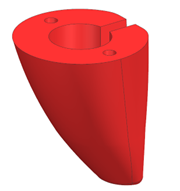
\includegraphics[width=3.5cm]{design/Droneleg.png} }}%
    \qquad
    \subfloat[\centering Mounted Motor]{{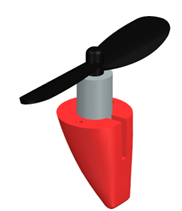
\includegraphics[width=3.5cm]{design/Dronepressfit.png} }}%
    \qquad
    \subfloat[\centering Prop Guard]{{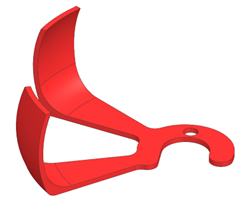
\includegraphics[width=3.5cm]{design/Dronepropguard.png} }}%
    \caption{3D-Printed drone parts}%
    \label{fig:example}%
\end{figure}

The project formulation states that the “Stress of the drone’s structural system should not exceed rupture point. System does not experience fracture”. This was tested through Ansys Mechanical Static Structural Analysis. Using the CAD model of the drone, the following boundary conditions were applied: Fixed constraint on the bottom area (excluding the drones arms), Z direction forces (upwards) was applied on each of the motor mount screw holes according to the found motor thrust, a single force vector in the Z direction (downwards) was applied to the top face (excluding the drones arms), to resemble the gravity force caused by the weight of the drone. Besides the boundary condition, the setup contained a mesh refinement of 3 steps, a material assignment of FR4 Fiber Glass Epoxy Board and a solution setting of equivalent stress. Below is a picture of the stress simulation of the initial design, which showed clear stress concentrations in the corners where the motor arms runs into the body section. The stress concentration had a magnitude of 1.6839 MPa which is satisfactory regarding the requirement of fracture, since the tensile strength of the given material is 320 MPa \cite{FR4}. 

\begin{figure}[H]%
    \centering
    \subfloat{{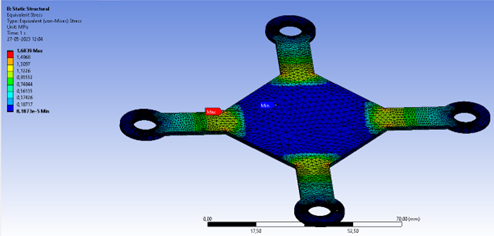
\includegraphics[width=10cm]{design/Ansys1.png} }}%
    \caption{Initial Ansys Simulation}%
    \label{fig:example}%
\end{figure}

Although it was clear that the drone body would be strong enough to operate under max power, the stress concentrations were undesirable. Therefore 20 mm radii was added to the stress all corner points of the drone body. Repeating the simulation with the same boundary conditions, it was clear that the added radii removed the stress concentrations and instead distributed the stress over a broader area of the motor arms. Furthermore, it was found that the maximum stress was found to be 0.87154 MPa, which is approximately half the maximum strength of the initial model that had the stress concentrations.

\begin{figure}[H]%
    \centering
    \subfloat{{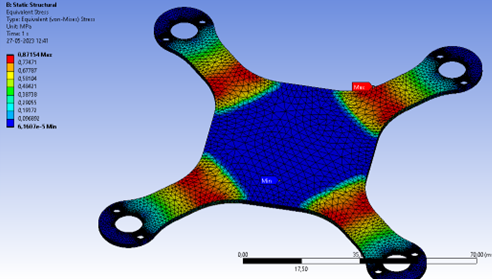
\includegraphics[width=10cm]{design/Ansys2.png} }}%
    \caption{Final Ansys Simulation}%
    \label{fig:example}%
\end{figure}

To power the drone a single cell Turnigy Li-Po battery is used, at 3.7 - 4.2 V and 300 mAh. The battery is chosen specifically to be able to supply the needed current of the drone. With a C-rating of 35C, the battery is able to discharge continously at 10.5 amps which is sufficent for the electrical circuit. The motors used are 8520 brushed Coreless DC-motors, which properties are characterized in the control chapter under thrust testing using the stock 2-bladed propellers that the motors were shipped with. 

\begin{figure}[H]%
    \centering
    \subfloat[\centering Turnigy Battery]{{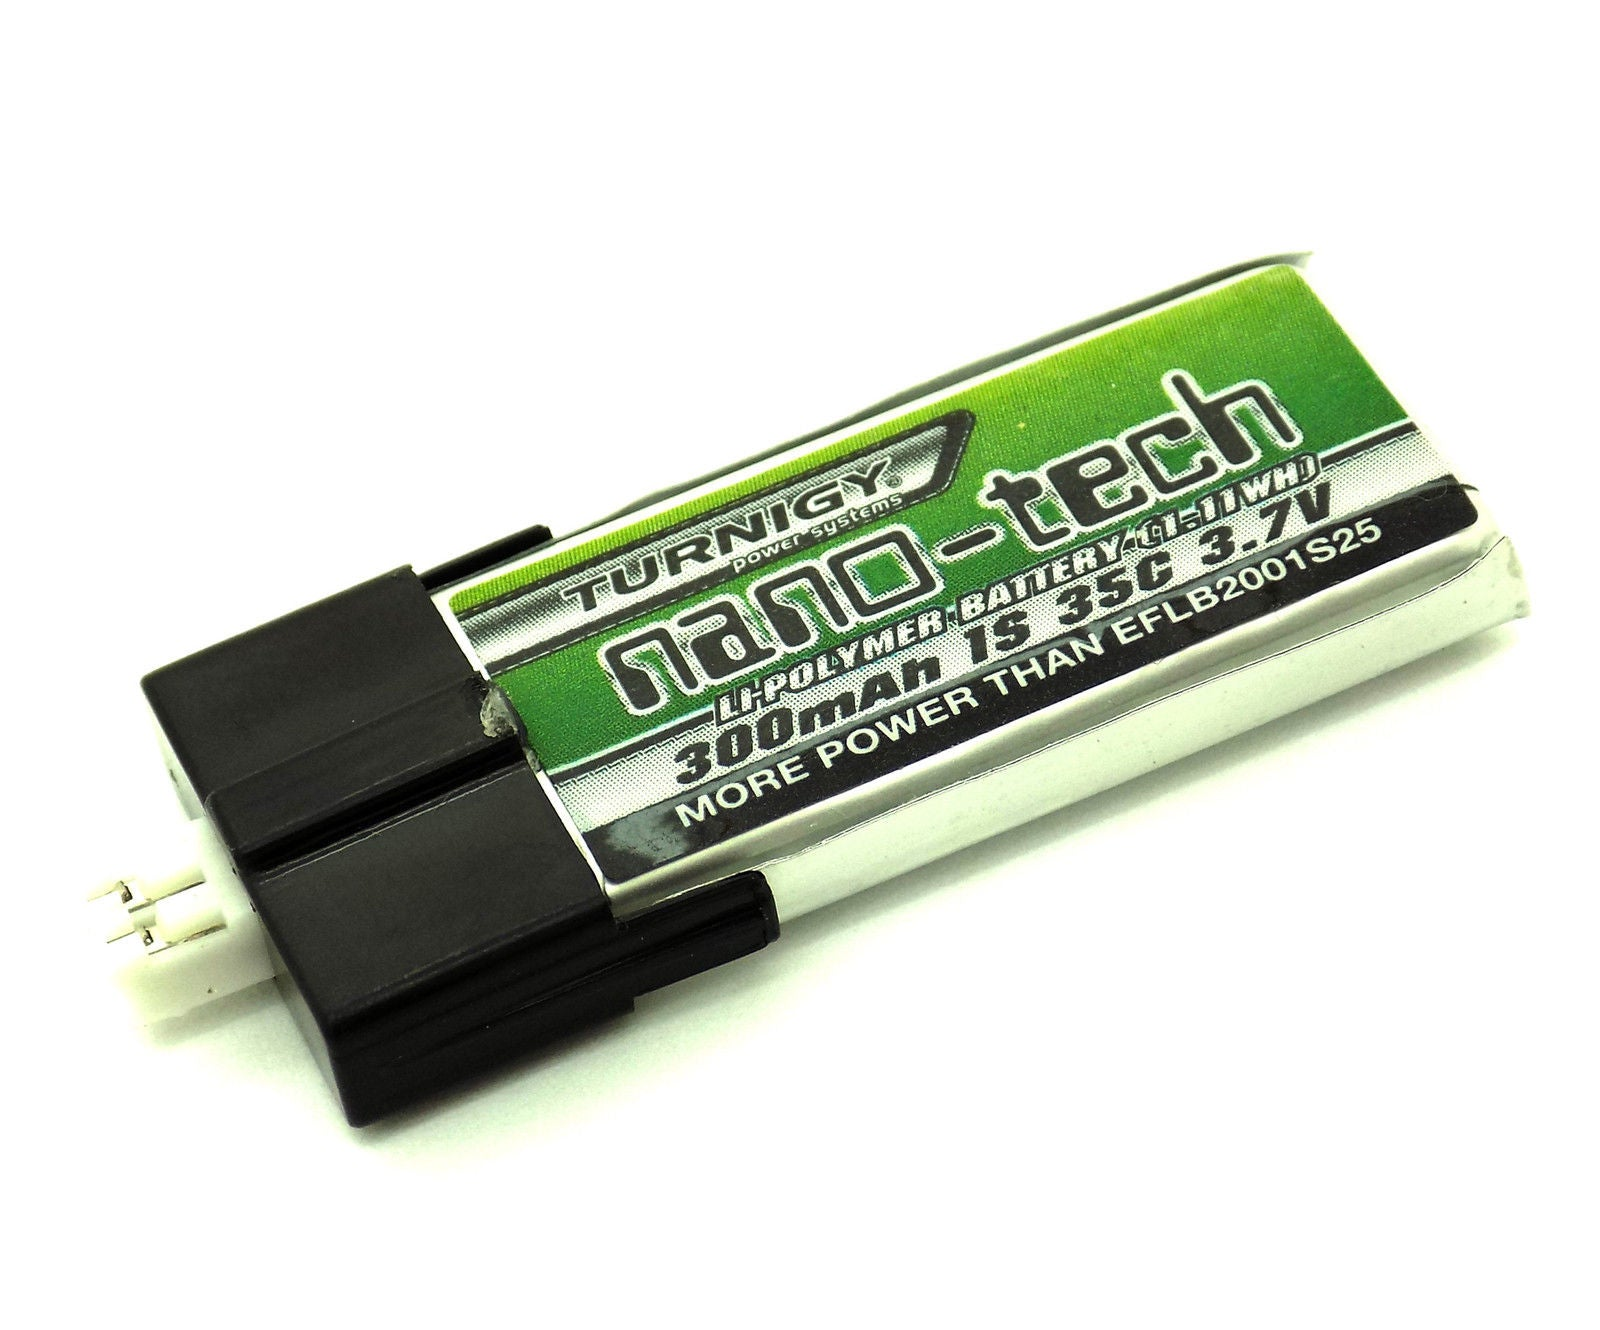
\includegraphics[width=5cm]{design/battery.jpeg} }}%
    \qquad
    \subfloat[\centering 8520 DC-motor]{{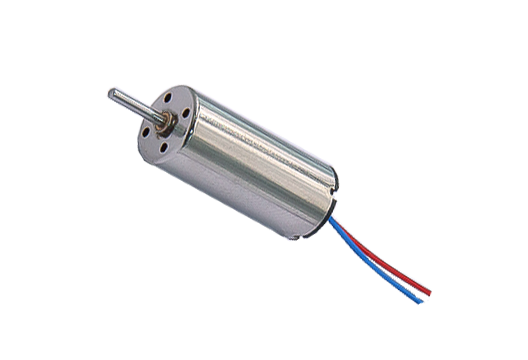
\includegraphics[width=5cm]{design/8520.jpg} }}%
    \caption{Motor and Battery used on the drone}%
    \label{fig:example}%
\end{figure}

After assembly of the drone including all the parts, it became apparent that the initial weight estimation of the drone was too low. After weighing the final physical setup it weighed 70 grams, XX grams over the intital estimation. This of course meant that the drones motors had less excess thrust than initially expected, meaning less control authority. In an attempt to mitigate this, the option of 3-bladed propellers were explored since they in theory would be able to provide extra thrust. The 3-bladed propellers were printed with SLA in the Tough 2000 resin on a Form 3 machine. Testing the new propellers in the same thrust setup used to characterize the motors using the 2-bladed propellers, it showed that the 3-bladed propellers produced 12 grams total extra (combining 4 motors), but also pulled a total of 4 amps extra. Since the battery used does not have the sufficient continous amp supply this option was not further explored, instead lightweighting options was used to reduce the total weight to 60 grams. In order to have an alitude feedback a GY-VL53L0XV2 ToF sensor was emplyed on the underside of the drone, to measure the drone-to-ground distance. In development a budget was created to ensure that the possibilty of achieving the project goals was always possible, the budget for the project can be found in appendix \ref{appendix_budget}.


\begin{figure}[H]%
    \centering
    \subfloat[\centering Motor Mount]{{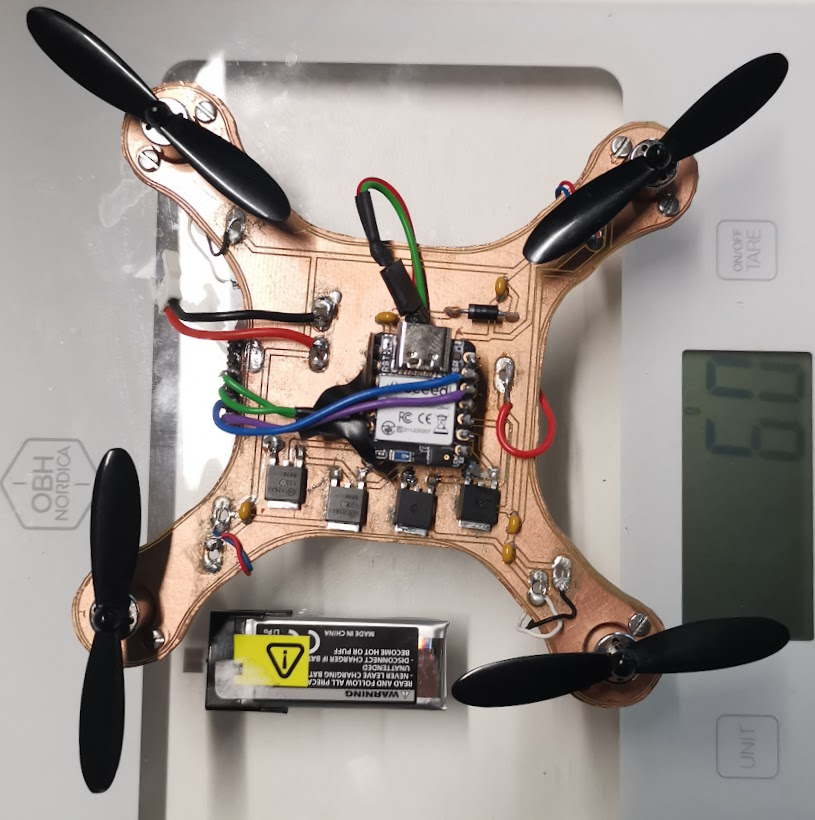
\includegraphics[width=3cm]{design/dronescale.jpg} }}%
    \qquad
    \subfloat[\centering Mounted Motor]{{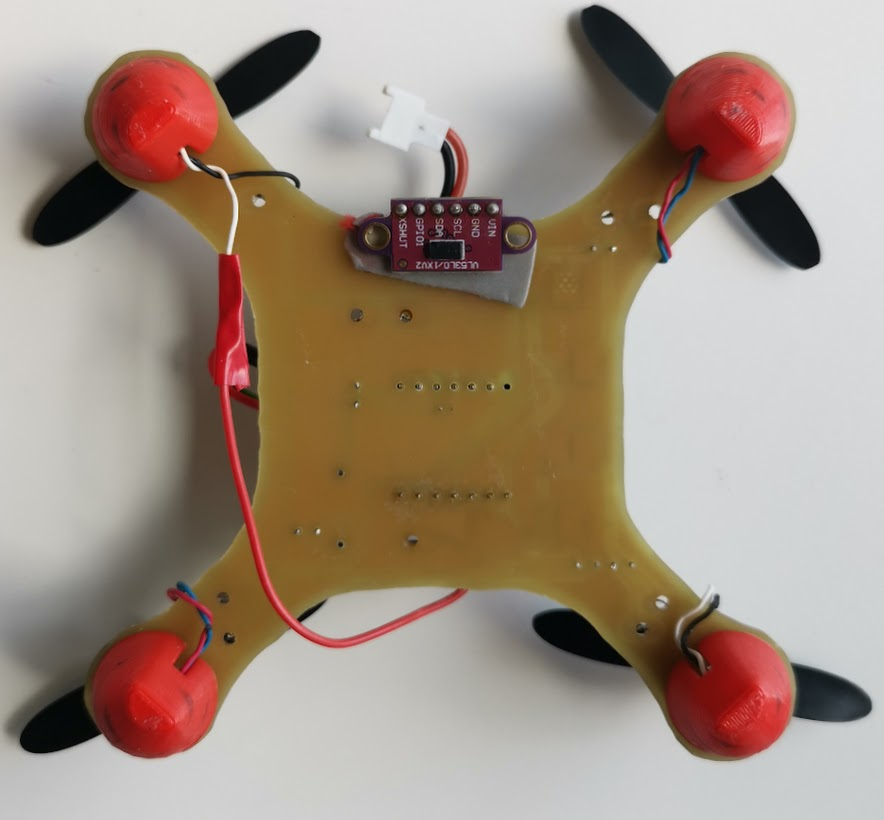
\includegraphics[width=3cm]{design/dronebottom.jpg} }}%
    \qquad
    \subfloat[\centering Prop Guard]{{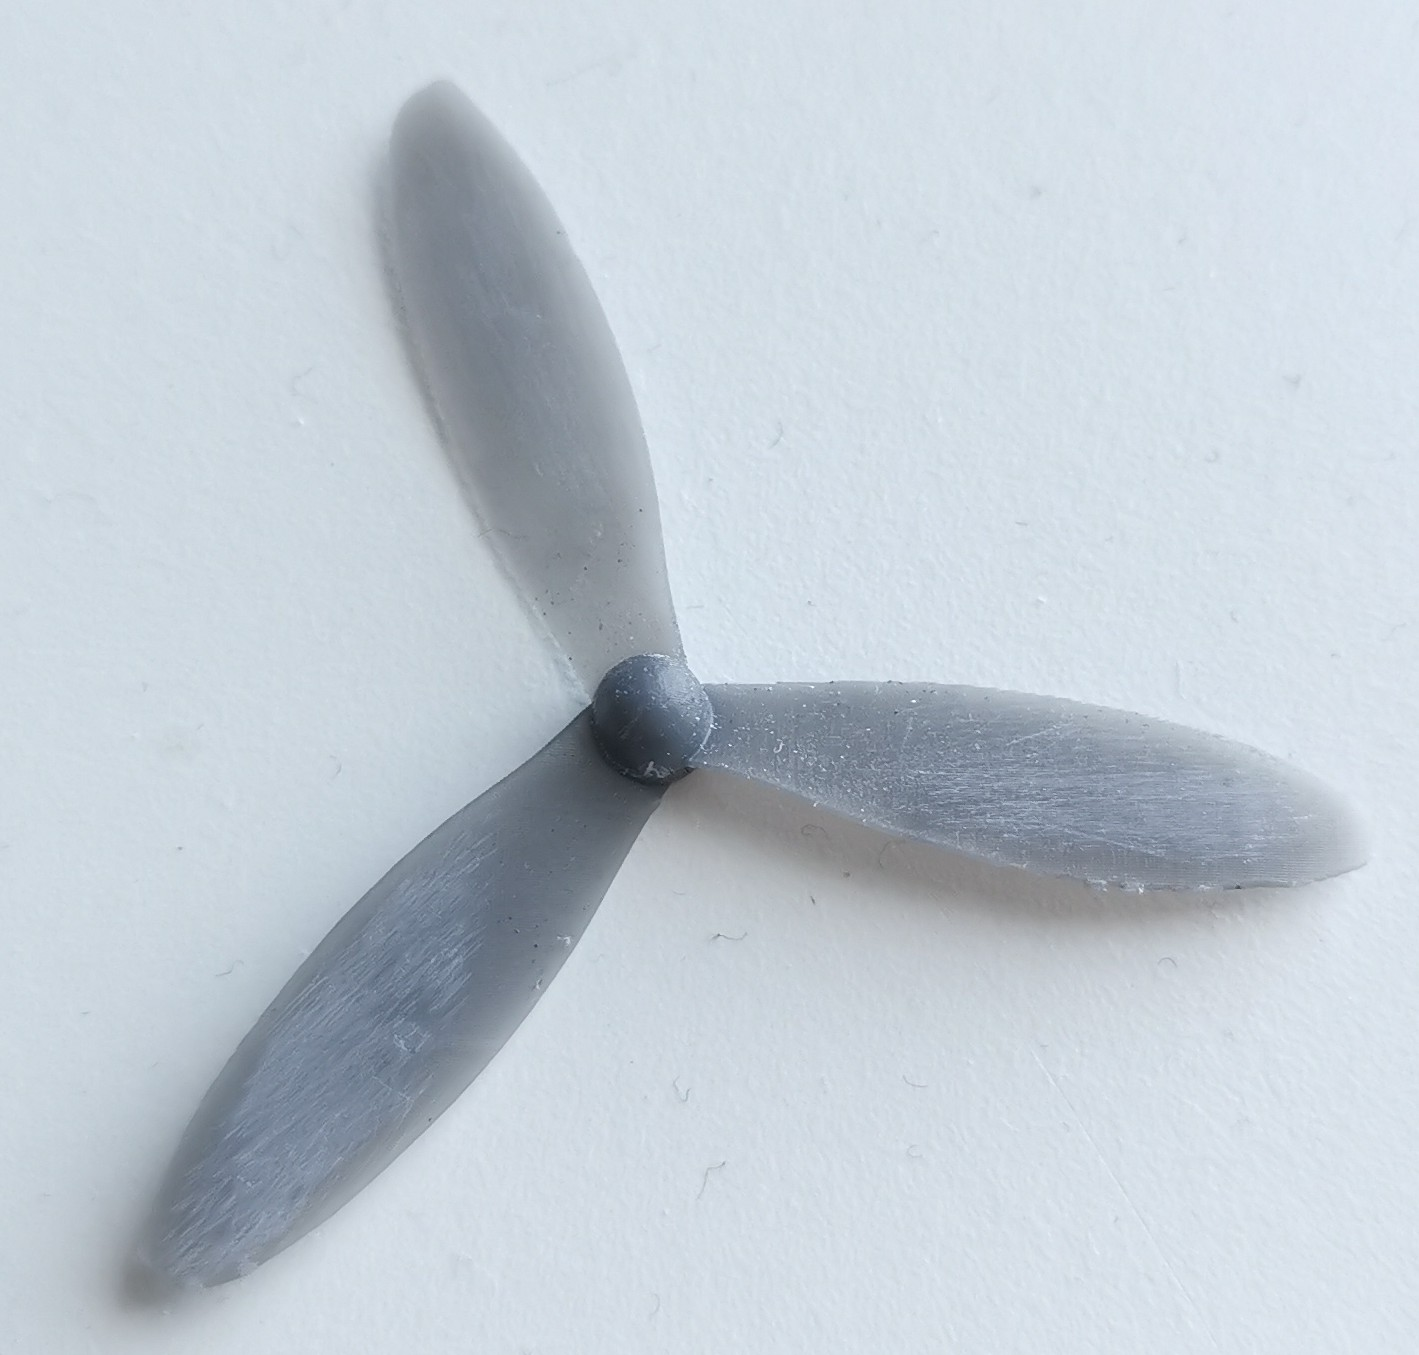
\includegraphics[width=3cm]{design/propthree.jpg} }}%
    \caption{3D-Printed drone parts}%
    \label{fig:example}%
\end{figure}